\def\duedate{11/17/21}
\def\HWnum{3}
% Document setup
\documentclass[12pt]{article}
\usepackage[margin=1in]{geometry}
\usepackage{fancyhdr}
\usepackage{lastpage}

\pagestyle{fancy}
\lhead{Richard Whitehill}
\chead{PHYS 714 -- HW \HWnum}
\rhead{\duedate}
\cfoot{\thepage \hspace{1pt} of \pageref{LastPage}}

% Encoding
\usepackage[utf8]{inputenc}
\usepackage[T1]{fontenc}

% Math/Physics Packages
\usepackage{amsmath}
\usepackage{amssymb}
\usepackage{dsfont}
\usepackage{mathtools}
\usepackage[arrowdel]{physics}
\usepackage{siunitx}

\AtBeginDocument{\RenewCommandCopy\qty\SI}

% Reference Style
\usepackage{hyperref}
\hypersetup{
    colorlinks=true,
    linkcolor=blue,
    filecolor=magenta,
    urlcolor=cyan,
    citecolor=green
}

\newcommand{\eref}[1]{Eq.~(\ref{eq:#1})}
\newcommand{\erefs}[2]{Eqs.~(\ref{eq:#1})--(\ref{eq:#2})}

\newcommand{\fref}[1]{Fig.~\ref{fig:#1}}
\newcommand{\frefs}[2]{Figs.~\ref{fig:#1}--\ref{fig:#2}}

\newcommand{\tref}[1]{Table~\ref{tab:#1}}
\newcommand{\trefs}[2]{Tables~\ref{tab:#1}-\ref{tab:#2}}

% Figures and Tables 
\usepackage{graphicx}
\usepackage{float}

\newcommand{\bef}{\begin{figure}[h!]\begin{center}}
\newcommand{\eef}{\end{center}\end{figure}}

\newcommand{\bet}{\begin{table}[h!]\begin{center}}
\newcommand{\eet}{\end{center}\end{table}}

% tikz
\usepackage{tikz}
\usetikzlibrary{calc}
\usetikzlibrary{decorations.pathmorphing}
\usetikzlibrary{decorations.markings}
\usetikzlibrary{arrows.meta}
\usetikzlibrary{positioning}

% tcolorbox
\usepackage[most]{tcolorbox}
\usepackage{xcolor}
\usepackage{xifthen}
\usepackage{parskip}

\newcommand*{\eqbox}{\tcboxmath[
    enhanced,
    colback=black!10!white,
    colframe=black,
    sharp corners,
    size=fbox,
    boxsep=8pt,
    boxrule=1pt
]}

% Miscellaneous Definitions/Settings
\newcommand{\prob}[2]{\textbf{#1)} #2}

\setlength{\parskip}{\baselineskip}
\setlength{\parindent}{0pt}

\def\complexs{\mathbb{C}}
\def\reals{\mathbb{R}}
\def\naturals{\mathbb{N}}
\def\integers{\mathbb{Z}}
\def\rationals{\mathbb{Q}}
\def\id{\mathds{1}}



\begin{document}
    
\prob{1}{
Given $A \in \complexs^{m \times n}$ with $m \geq n$, show that $A^{*}A$ is nonsingular if and only if $A$ has full rank.
}

Recall that $A$ is full rank if $\rank(A) = \min\{m,n\} = n$.
Additionally, note that $\rank(A^{*}A) = \rank(A)$.

Let us prove the forward direction first.
Suppose that $A^{*}A$ is a nonsingular matrix, meaning that its eigenvalues are nonzero (otherwise its determinant would be zero).
Hence, $A$ has $n$ nonzero singular values, or equivalently $\Sigma$ has $n$ nonzero diagonal entries, which implies that $A$ has rank $n$ since $\rank(A) = \rank(U \Sigma V^{\rm T}) = \rank(\Sigma) = n$, where we used the fact that $U$ and $V$ are invertible matrices.

Now, suppose that $A$ is full rank.
Then, since $A$ has a singular value decomposition
\begin{eqnarray}
    \label{eq:A*A-SVD}
    A^{*}A = V \Sigma^2 V^{*} 
,\end{eqnarray}
which implies that 
\begin{eqnarray}
    \label{eq:determinant-A*A}
    \det(A^{*}A) = \det(\Sigma^2) = \prod_{i=1}^{n} \sigma_{i}^2 \ne 0
,\end{eqnarray}
where the last inequality comes from the fact that $\rank(\Sigma) = \rank(A) = n$, implying that $\Sigma$ has $n$ nonzero singular values.
Thus, we have shown that $A^{*}A$ is nonsingular.


\prob{2}{
For the matrix 
\begin{eqnarray}
\label{eq:A-2} 
    A = \begin{pmatrix}
    3 & 4 \\
    0 & 1 \\
    4 & 0
    \end{pmatrix}
\end{eqnarray}
}

a) Find the Householder matrix $\rm H$

We calculate the Householder matrix as follows.
Denote $A = \begin{pmatrix} a_1 a_2 \end{pmatrix}$, where $a_1 = \begin{pmatrix} 3 & 0 & 4 \end{pmatrix}^{\rm T}$ and $a_2 = \begin{pmatrix} 4 & 1 & 0 \end{pmatrix}^{\rm T}$.
Our first reflection matrix is constructed as follows such that $a_1 \rightarrow ||a_1||_{2} e_1$under $H_1$.
Observe that $||a_1|| = 5$ and let 
\begin{eqnarray}
    \label{eq:u1}
    u_1 = a_1 + 5e_1 = \begin{pmatrix}
    8 \\ 0 \\ 4
    \end{pmatrix}
.\end{eqnarray}
Then
\begin{eqnarray}
    \label{eq:H1}
    H_1 = \id_{3 \times 3} - \frac{2}{||u||^2} u u^{\rm T} = \begin{pmatrix}
    1 & 0 & 0 \\
    0 & 1 & 0 \\
    0 & 0 & 1
    \end{pmatrix}
    - \frac{2}{5}\begin{pmatrix}
    2 \\ 0 \\ 1 
    \end{pmatrix}
    \begin{pmatrix}
    2 & 0 & 1   
    \end{pmatrix}
    = \begin{pmatrix}
        -3/5 & 0 & -4/5 \\
        0 & 1 & 0 \\
        -4/5 & 0 & 3/5
    \end{pmatrix}
,\end{eqnarray}
and
\begin{eqnarray}
    \label{eq:A-after-ref1}
    A \rightarrow H_1 A = \begin{pmatrix}
        -5 & -12/5 \\
        0 & 1 \\
        0 & -16/5
    \end{pmatrix}
.\end{eqnarray}

Now, we repeat a similar process for the second column.
We let $\tilde{a}_{2} = \begin{pmatrix} 1 & -16/5 \end{pmatrix}^{\rm T}$, and 
\begin{eqnarray}
    \label{eq:u2}
    u = \tilde{a}_{2} + {\rm sign}(1)e_{1} = \begin{pmatrix}
    1 + \sqrt{281}/5 \\ -16/5
    \end{pmatrix}
.\end{eqnarray}
Hence,
\begin{eqnarray}
    \label{eq:H2}
    H_2 = \begin{pmatrix}
        1 & 0 \\
        0 & \id - 2 \hat{u} \hat{u}^{\rm T} 
    \end{pmatrix}
    = \begin{pmatrix}
        1 & 0 & 0 \\
        0 & -5/\sqrt{281} & 16/\sqrt{281} \\
        0 & 16/\sqrt{281} & 5/\sqrt{281}
    \end{pmatrix}
.\end{eqnarray}
Finally, we have 
\begin{eqnarray}
    \label{eq:H2H1A}
    H_1 A \rightarrow H_2 H_1 A = \begin{pmatrix}
    -5 & -12/5 \\
    0 & -\sqrt{281}/5 \\
    0 & 0 
    \end{pmatrix}  
.\end{eqnarray}
The full reflection matrix $H = H_2 H_1$ is as follows:
\begin{eqnarray}
    \label{eq:H-mat}
    H = \begin{pmatrix}
        -3/5 & 0 & -4/5 \\
        -64\sqrt{281}/1405 & -5\sqrt{281}/281 & 48\sqrt{281}/1405 \\
        -4\sqrt{281}/281 & 16\sqrt{281}/281 & 3\sqrt{281}/281
    \end{pmatrix}
.\end{eqnarray}


b) Use (a) to calculate QR decomposition

With the above work, we can calculate the QR decomposition simply.
The matrix $R$ is just the upper triangular matrix
\begin{eqnarray}
    \label{eq:R-mat}
    R = \begin{pmatrix}
        -5 & -12/5 \\
        0 & -\sqrt{281}/5
    \end{pmatrix}
,\end{eqnarray}
and 
\begin{eqnarray}
    \label{eq:Q-mat}
    Q = (H_2 H_1)^{-1} = (H_2 H_1)^{\rm T} = H_1^{\rm T} H_2^{\rm T} = \begin{pmatrix}
        -3/5 & -64\sqrt{281}/1405 & -4\sqrt{281}/281 \\
        0 & -5\sqrt{281}/281 & 16\sqrt{281}/281 \\
        -4/5 & 48\sqrt{281}/1405 & 3\sqrt{281}/281
    \end{pmatrix} 
.\end{eqnarray}
Note that we remove the last column such that $Q$ has the same shape as $A$:
\begin{eqnarray}
    \label{eq:Q-mat-proper}
    Q = \begin{pmatrix}
        -3/5 & -64\sqrt{281}/1405 \\
        0 & -5\sqrt{281}/281 \\
        -4/5 & 48\sqrt{281}/1405
    \end{pmatrix} 
.\end{eqnarray}



\prob{3}{
Let $A = U \Sigma V^{\rm T} \in \reals^{m \times n} ~ (m \geq n)$ with singular values $\sigma_1 \geq \sigma_2 \geq \ldots \geq \sigma_{n}$.
Prove $||A||_{2} = \sigma_1$.
Moreover, if $A$ is square and nonsingular, then $||A^{-1}||_{2}^{-1} = \sigma_{n}$ and $\kappa_2(A) = \sigma_1 / \sigma_{n}$.
}

Recall that $||A||_{2} = \sqrt{\rho(A^{\rm T}A)}$, where $\rho(A^{\rm T}A)$ is the spectral radius of $A$.
The eigenvalues of $A^{\rm T}A$ just the square of the singular values of $A$, so by definition
\begin{eqnarray}
    \label{eq:spectral-radius}
    ||A||_{2} = \sqrt{\rho(A^{\rm T}A)} = \sqrt{\sigma_1^2} = \sigma_1
.\end{eqnarray}

If $A$ is $n \times n$ and nonsingular, then all of its singular values are nonzero (i.e. $\Sigma$ is invertible).
This can be observed as follows.
Since $A$ is nonsingular, then $A^{\rm T}A$ is nonsingular since $\det(A^{\rm T}A) = \det^2(A) \ne 0$.
Hence, this means that all the eigenvalues of $A^{\rm T}A$ are nonzero (otherwise its determinant would be zero), and therefore the singular values of $A$ are nonzero.
Thus, 
\begin{eqnarray}
    \label{eq:Ainvs}
    A^{-1} = V \Sigma^{-1} U^{\rm T} 
,\end{eqnarray}
where $\Sigma_{ii}^{-1} = 1/\sigma_{i}$ for $i = 1,2,\ldots,n$ and $\Sigma_{ij}^{-1} = 0$ if $i \ne j$.
Notice that the ordering of the singular values of $A$ implies that $1/\sigma_{n} \geq \ldots \geq 1/\sigma_2 \geq 1/\sigma_1$, implying that the largest singular value of $A^{-1}$ is $1/\sigma_{n}$.
By the same work as above then
\begin{eqnarray}
    \label{eq:spectral-radius-Ainvs}
    ||A^{-1}||_{2} = \frac{1}{\sigma_{n}} \Leftrightarrow ||A^{-1}||_{2}^{-1} = \sigma_{n}
.\end{eqnarray}
Finally, we observe that for a square nonsingular matrix
\begin{eqnarray}
    \label{eq:condition-number}
    \kappa_{2}(A) = ||A^{-1}||_{2}||A||_{2} = \frac{\sigma_1}{\sigma_{n}} 
.\end{eqnarray}



\prob{4}{
Assume $A$ is singular, and $x$ is the solution to
\begin{eqnarray}
    \label{eq:minx}
    \min_{x} ||Ax - b||_{2} 
.\end{eqnarray}
Let $A = U \Sigma V^{\rm T}$ have rank $r < n$ and its SVD can be written as
\begin{eqnarray}
    \label{eq:A-SVD}
    A = \begin{bmatrix}
        U_1 & U_2
    \end{bmatrix}
    \begin{bmatrix}
        \Sigma_1 & 0 \\
        0 & 0
    \end{bmatrix}
    \begin{bmatrix}
        V_1^{\rm T} \\ V_2^{\rm T}
    \end{bmatrix}
.\end{eqnarray}
where $\Sigma_1$ is $r \times r$ nonsingular, and $U_1$, $V_1$ have $r$ columns.
Prove all solutions $x$ can be written as $x = V_1 \Sigma_1^{-1}U_1^{\rm T}b + V_2 z$, with $z$ is an arbitrary vector.
}

We proved in class that the vector $x$ which minimizes this norm is $x = V \Sigma^{-1} U^{\rm T}b$.
Written in terms of $U_{1,2}$, $V_{1,2}$, and $\Sigma_1$, we find that
\begin{eqnarray}
    \label{eq:solve-x}
    x = 
    \begin{pmatrix}
        V_1 & V_2 
    \end{pmatrix}  
    \begin{pmatrix}
        \Sigma_1^{-1} & 0 \\
        0 & 0
    \end{pmatrix}
    \begin{pmatrix}
    U_1^{\rm T} \\ U_2^{\rm T}
    \end{pmatrix}
    b 
    =
    V_1 \Sigma_1^{-1} U_1^{\rm T}b
.\end{eqnarray}
However, note that since $A$ has rank $r$, the kernel (or nullspace) of $A$ has dimension $n - r$, where $A (V_2 z) = 0$ for any vector $z$.
This can be observed by noting that $V$ is an orthogonal matrix, and since $A = U_1 \Sigma_1 V_1^{\rm T}$, then it follows that $A V_2 = 0$ since $V_1^{\rm T} V_2 = 0$.
Hence, the vector $x = V_1 \Sigma_1^{-1} U_1^{\rm T} b + V_2 z$ is also a vector which minimizes the norm above.


\prob{5}{
Consider
\begin{eqnarray}
    \label{eq:label}
    A = \begin{pmatrix}
        2 & 1 \\
        1 & 1 \\
        2 & 1
    \end{pmatrix}
    \quad
    b = \begin{pmatrix}
    12 \\ 6 \\ 18    
    \end{pmatrix}
.\end{eqnarray}
Write codes to solve the linear least square problem $Ax = b$ using (a) normal equation methods; (b) QR decomposition with modified Gram-Schmidt orthogonalization; (c) SVD decomposition.
}

For each method, the script is displayed along with a screenshot of the output:

a)

\inputpython{prob5a.py}
\begin{center}
    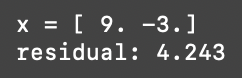
\includegraphics[width=0.3\textwidth]{prob5a.png} 
\end{center}

b)

\inputpython{prob5b.py}
\begin{center}
    
\includegraphics[width=0.3\textwidth]{prob5b.png} 
\end{center}

c)

\inputpython{prob5c.py}
\begin{center}
    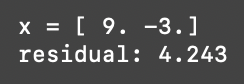
\includegraphics[width=0.3\textwidth]{prob5c.png} 
\end{center}



\end{document}
